%\section{Case Study: System-Level \\ Integration}
\section{Gemmini Case Studies}\label{sec:casestudies}
This section demonstrates how Gemmini enables full system co-design with two case studies. We use Gemmini to design a novel virtual address translation scheme, and to find the optimal SoC-level resource partition scheme of a multi-core, multi-accelerator system.

\subsection{Virtual Address Translation}
\label{virtual-memory-case-study}

% Point of this paragraph: We need a framework to co-design accelerators together with the virtual memory system.
With an RTL-level implementation that supports virtual memory, users can co-design their own virtual address translation schemes based on their accelerator and SoC configuration. Prior works in virtual address translation for DNN accelerators have proposed very different translation schemes, from NeuMMU~\cite{neummu-asplos2020}, which calls for a highly parallel address-translation system with 128 page-table walkers (PTWs), to Cong et al.~\cite{address-trans-cong-hpca2017}, who recommend a more modest two-level TLB hierarchy, with the host CPU's default PTW co-opted to serve requests by the accelerator. This lack of convergence in the prior literature motivates a platform that allows co-design and design-space exploration of the accelerator SoC together with its virtual address translation system, for both hardware designers and researchers. Fortunately, with Gemmini, we can iterate over a variety of address translation schemes as we tune the accelerator and SoC.

% Point of this paragraph: Describe our experimental setup
To demonstrate, we configure Gemmini to produce a two-level TLB cache, with one private TLB for the accelerator, and one larger shared TLB at the L2 cache that the private TLB falls back on when it misses. Our design includes only one PTW, shared by both the CPU and the accelerator, which is suitable for low-power devices. We configure the accelerator for low-power edge devices, with a 16-by-16 systolic mesh and a 256 KB scratchpad. As shown in Figure~\ref{fig:tlb_wait_cycles}, we iterate over a variety of TLB sizes to find the design that best balances TLB overhead and overall performance, including over a design point where the shared L2 TLB has zero entries.

% Point of this paragraph: The private TLB gives you much more bang-for-your-buck than the L2 TLB.
Figure~\ref{fig:tlb_wait_cycles} demonstrates that the private accelerator TLB has a far greater impact on end-to-end performance than the much larger shared L2 TLB. Increasing the private TLB size from just four to 16 improves performance by up to 11\%. However, adding even 512 entries to the L2 TLB never improves performance by more than 8\%. This is because our workloads exhibit high page locality; even with tiled workloads, our private TLB's hit rate remained above 84\%, even with the smallest TLB sizes we evaluated. In fact, we found that 87\% of consecutive \textit{read} TLB requests, and 83\% of consecutive \textit{write} TLB requests, were made to the same page number, demonstrating high page locality. However, because reads and writes were overlapped, read and write operations could evict each other's recent TLB entries.

\begin{figure}
    \centering
    \begin{subfigure}[t]{0.439\linewidth}
        \centering
        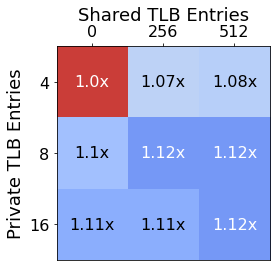
\includegraphics[width=\linewidth]{fig/tlb_entries.png}
        \caption{Without filter registers.}
        \label{fig:tlb_wait_cycles}
    \end{subfigure}
    \hfill
    \begin{subfigure}[t]{0.439\linewidth}
        \centering
        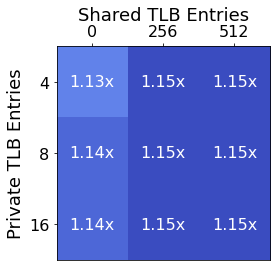
\includegraphics[width=\linewidth]{fig/tlb_entries_with_filter.png}
        \caption{With filter registers.}
        \label{fig:tlb_wait_cycles_with_filter}
    \end{subfigure}
    \caption{Normalized performance of ResNet50 inference on Gemmini-generated accelerator with different private and shared TLB sizes.}
    \vspace{-0.2in}
\end{figure}

% Point of this paragraph: On top of tuning the TLB sizes, we can make small optimizations to the virtual address translation system.
Although tuning TLB sizes improves hit rates, our private TLB hit latency in the tests shown in Figure~\ref{fig:tlb_wait_cycles} was still several cycles long. Fortunately, using the Gemmini platform, we were able to implement a simple optimization: a single register that caches the last TLB hit for read operations, and another register that caches TLB hits for write operations. These two registers allow the DMA to ``skip'' the TLB request if two consecutive requests are made to the same virtual page number, and help reduce the possibility of read-write contention over the TLB. These ``filter registers'' reduce the TLB hit latency to 0 cycles for consecutive accesses to the same page. As Figure~\ref{fig:tlb_wait_cycles_with_filter} shows, this low-cost optimization significantly improves our end-to-end performance, especially for small private TLB sizes. Due to our high TLB hit rate and low TLB hit penalty, we found that a very small 4-entry private TLB equipped with filter registers, but without an expensive shared L2 TLB, achieved only 2\% less than the maximum performance recorded. With such a configuration, the private TLB hit rate (including hits on the filter registers) reached 90\% and further increases to either TLB's size improved performance by less than 2\%, even if hundreds of new TLB entries were added.
% the total number of cycles spent by the DMA waiting for a TLB response only reached \textcolor{red}{X\%} of the total end-to-end runtime, showing that the virtual address translation scheme was no longer a primary performance bottleneck.

Using Gemmini, we have demonstrated that a modest virtual address translation system, with very small private TLBs, a single page-table-walker, and two low-cost filter registers for the TLB, can achieve near maximum performance for low-power edge devices. Gemmini is designed to enable such co-design of the SoC and its various components, such as its virtual address translation system.


\subsection{System-Level Resource Partition}
\label{cache-contention}

%We have better system-level integration than anyone else. There is a push-button flow to generate RTL for an entire SoC, including a RISC-V CPU, a TileLink interconnect, cache hierarchy, etc.

%This system-level integration allows us to perform an apples-to-apples comparison to state-of-the-art accelerators like NVDLA, to whom we will \textbf{hopefully} be competitive by publication time.

%Gemmini uses the RoCC interface of the Rocket Chip
%SoC generator and a TileLink memory port to communicate with a host processor system. Gemmini is also a part of Chipyard integrated SoC research
%and development framework~\cite{chipyard}, which provides it with a broader digital design environment which includes additional IP components, FPGA-accelerated simulation using the FireSim~\cite{karandikar2018firesim} platform, and VLSI implementation flows. The integration with the Chipyard enables a broad spectrum of high fidelity evaluation and experimentation with Gemmini.

% \textbf{Paragraphs:}
% \begin{enumerate}
%     \item Gemmini enables application-system co-design.
%     \item Real-world DNN applications, such as ResNet50, have diverse layer types which react to system configurations in different ways
%     \item Experimental setup
%     \item As shown in Figure X, layers with higher arithmetic intensity benefit more from a bigger scratchpad. Memory-bound layers, like resadds, are unaffected in the single-core case
%     \item However, in the dual core case, residual addition layers benefit very much from higher cache sizes
%     \item This demonstrates that memory partitioning schemes must be co-designed with the application in order to achieve maximum performance.
% \end{enumerate}

% Point of this paragraph: Gemmini enables application-system co-design.

Gemmini also enables application-system co-design for real-world DNN workloads. To demonstrate, we present a case study describing a system-level design decision: memory partitioning based on application characteristics. We investigate memory partitioning strategies in both single-core and multi-core SoCs.

% Point of this paragraph: Real-world DNN applications, such as ResNet50, have diverse layer types which react to system configurations in different ways

\begin{figure*}[t]
\centering
\begin{subfigure}[b]{0.325\textwidth}
    % \vspace{23pt}
    \centering
    \scalebox{0.875} {
    \begin{tabular}{ l | c | c | c }
    \hline
    \makecell{Config\\Name} & \makecell{Scratchpad\\(per core)} & \makecell{Accumulator\\(per core)} & \makecell{L2\\Cache} \\  
    \hline
    \hline
    Base & 256 KB & 256 KB & 1 MB   \\
    BigSP & 512 KB & 512 KB & 1 MB  \\
    BigL2 & 256 KB & 256 KB & 2 MB  \\ \hline
    \multicolumn{1}{c}{} & \multicolumn{1}{c}{} & \multicolumn{1}{c}{} & \multicolumn{1}{c}{} \\
    \end{tabular}
    }
    \caption{Resource contention SoC configurations}
    \label{tab:contention-soc-configs}
\end{subfigure}
\hfill
\begin{subfigure}[b]{.325\textwidth}
    \vspace{0pt}
      \centering
      % include first image
      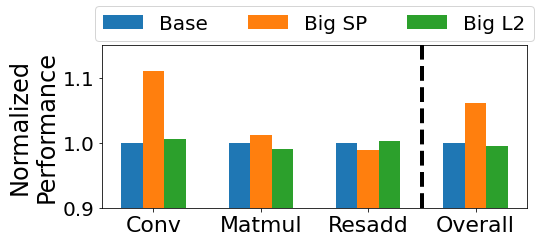
\includegraphics[width=\linewidth]{fig/single-core-contention.png}
      \caption{Performance of single-core SoCs.}
      \label{fig:single-contention}
\end{subfigure}
\hfill
\begin{subfigure}[b]{.325\textwidth}
    \vspace{0pt}
      \centering
      % include first image
      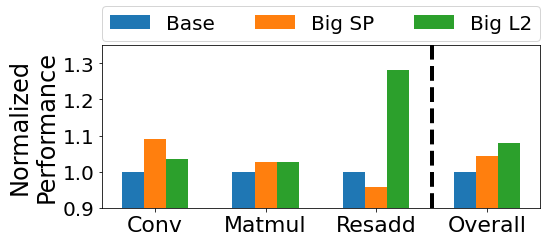
\includegraphics[width=\linewidth]{fig/dual-core-contention.png}
      \caption{Performance of dual-core SoCs.}
      \label{fig:dual-contention}
\end{subfigure}
    \caption{Performance of the various SoC configurations in the case study, normalized to the performance of the Base configuration.}
    \label{fig:contention}
    \vspace{-0.2in}
\end{figure*}

Real-world DNN applications, such as CNN inference, have diverse layer types which have different computational requirements and which contend for resources on an SoC in different ways. For example, ResNet50 includes convolutions, matrix multiplications, and residual additions, which all exhibit quite different computational patterns. Convolutions have high arithmetic intensity; matrix multiplications have less; and residual additions have almost no data re-use at all. Additionally, unlike the other two types of layers, residual additions benefit most if layer outputs can be stored inside the cache hierarchy for a long time, rather than being evicted by intermediate layers, before finally being consumed several layers later. These different layer characteristics suggest different ideal SoC configurations. To run with optimal performance over an entire DNN, a hardware designer must balance all these constraints.

% \begin{table}[t]
% \centering
% \begin{tabular}{ l | c | c | c | c }
% \hline
% Config Name & Cores & \makecell{Scratchpad\\(per core)} & \makecell{Accumulator\\(per core)} & \makecell{L2 Cache} \\  
% \hline
% \hline
% Base-Single & 1 & 256 KB & 256 KB & 1 MB   \\
% Base-Dual & 2 & 256 KB & 256 KB & 1 MB   \\
% BigSP-Single & 1 & 512 KB & 512 KB & 1 MB  \\
% BigSP-Dual & 2 & 512 KB & 512 KB & 1 MB  \\
% BigL2-Single & 1 & 256 KB & 256 KB & 2 MB   \\
% BigL2-Dual & 2 & 256 KB & 256 KB & 2 MB   \\ \hline
% \end{tabular}
% \caption{Resource contention SoC configurations}
% \label{tab:contention-soc-configs}
% \end{table}

% Point of this paragraph: Experimental setup

To demonstrate, we run ResNet50 inference on six different SoC configurations. These are the three different configurations described in Figure~\ref{tab:contention-soc-configs}, repeated for both single- and dual-core SoCs (as in Figure~\ref{fig:contention-soc}), where each CPU core has its own Gemmini-generated accelerator. The dual-core SoCs run two ResNet50 workloads in parallel, while the single-core SoCs run just one. The base design point has a 256 KB scratchpad, and a 256 KB accumulator per core, as well as a 1 MB shared L2 cache. The scratchpad and accumulator memories are private to the accelerators, but the L2 cache is shared by all CPUs and accelerators on the SoC. We presume that we have 1 MB of extra SRAM that we can allocate to our memory system, but we need to decide whether to allocate these SRAMs to the accelerators' private memory, or to the L2 caches.

% Point of this paragraph: As shown in Figure X, layers with higher arithmetic intensity benefit more from a bigger scratchpad. Memory-bound layers, like resadds, are unaffected in the single-core case

As shown in Figures~\ref{fig:single-contention} and~\ref{fig:dual-contention}, convolutional layers benefit from a larger, explicitly managed scratchpad, due to their very high arithmetic intensity. Convolutional kernels exhibit a 10\% speedup with one core, and an 8\% speedup in the dual-core case, when the scratchpad and accumulator memory is doubled by the addition of our 1 MB worth of SRAMs. The matmul layers, on the other hand, achieve only a 1\% and 3\% speedup when the scratchpad is enlarged in the single-core and dual-core cases respectively, due to their lower arithmetic intensity. Residual additions, which have virtually no data re-use and are memory-bound operations, exhibit no speedup when increasing the scratchpad memory size. Instead, they exhibit a minor 1\%-4\% slowdown, due to increased cache thrashing. In the single-core case, the increased convolutional and matrix multiplication performance is enough to make the design point with increased scratchpad memory, rather than increased L2 memory, the most performant design point.

% Point of this paragraph: However, in the dual core case, residual addition layers benefit very much from higher cache sizes

However, Figure~\ref{fig:dual-contention} shows that when we run dual-process applications that compete for the same shared L2 cache, allocating the extra 1~MB of memory to the shared L2 cache improves overall performance more than adding that memory to the accelerators' scratchpad and accumulator memories. Increasing the scratchpad size still improves convolutional performance more than increasing the L2 size, but this improvement in performance is more than negated by the 22\% speedup of residual additions that the dual-core BigL2 design point enjoys. This is because each core's residual addition evicts the input layer that the other one is expecting from the shared L2 cache, increasing the latency of memory-bound residual addition layers. The dual-core BigL2 configuration, which increases the shared cache sizes, alleviates this contention, reducing the L2 miss rate by 7.1\% over the full ResNet50 run, and increasing overall performance by 8.0\%. The BigSP configuration, on the other hand, improves overall performance by only 4.2\% in the dual-core case.

% Point of this paragraph: This demonstrates that memory partitioning schemes must be co-designed with the application in order to achieve maximum performance.

With Gemmini, we have demonstrated how the memory partitioning strategy, a key component of system-level design, can be decided based upon application characteristics, such as the composition of layer types and the number of simultaneous running processes.

%%%%%%% OLDER VERSION

% We demonstrate an example of the benefits of Gemmini's system integration by studying a system-level design decision: memory partitioning.
% Recent work~\cite{kelp} observed how host memory bandwidth contention challenges affect cloud-based machine learning accelerators (specifically, the Google TPU) in which the CPU is shared by multiple applications. In this case, the host CPU memory bandwidth is a resource under contention, since multiple CPU applications require access to memory, as well as the application running on the accelerator.

% We use Gemmini to study whether different memory partitioning design choices can impact similar resource-contention scenarios in tightly integrated edge devices. The SoC architecture under evaluation is a dual-core application processor, in which each core has a dedicated Gemmini accelerator tightly integrated with it. Therefore, the system has a total of two host processors and two Gemmini accelerators. In this SoC architecture, a shared last-level cache (L2) is shared by both the host CPUs and the accelerators, as shown in Figure~\ref{fig:contention-soc}.

%\begin{figure}
%    \centering
%    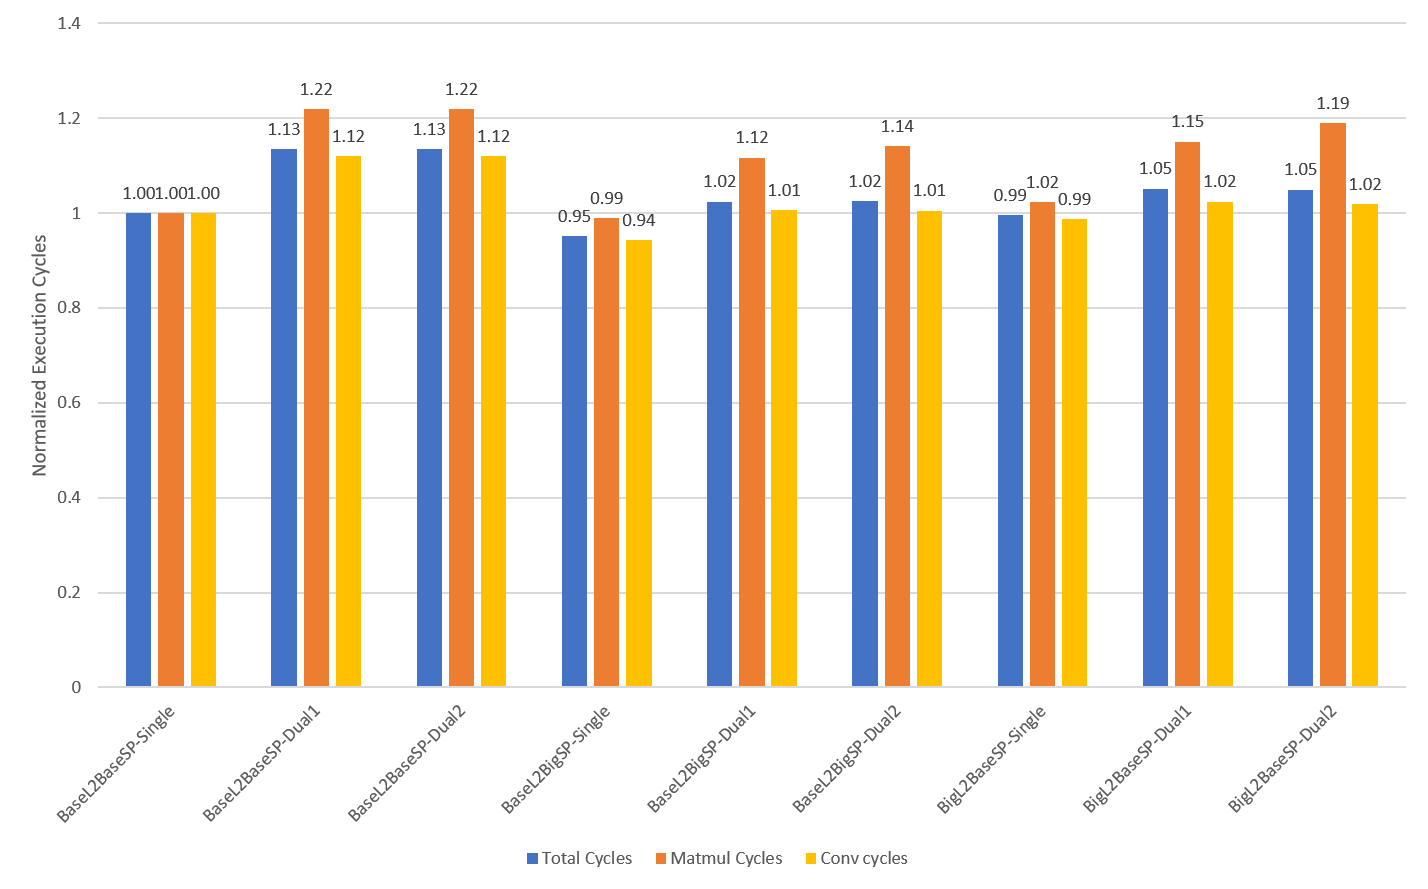
\includegraphics[width=1\linewidth]{fig/contention-normalized-perf.png}
%    \caption{Normalized execution cycles of the three SoC configurations in the last-level cache resource contention case study. For each of the three SoC configurations, the normalized execution cycles are presented for each of the ResNet-50 inference application, on each core. The execution cycles are normalized to the single-core execution of the base configuration.}
%    \label{fig:contention-cycles}
%\end{figure}


% When both application cores and Gemmini accelerators are running workloads concurrently, we would expect contention over the shared L2 to impact the execution time of each workload, compared to running the same workload on a single core individually. 
%We would also expect this phenomenon to occur when running applications which utilize the Gemmini accelerators, since their memory backend is also connected to the shared L2.

% We confirm the L2 contention expectation by measuring the performance of a ResNet50 inference application on a single core using Gemmini, and measuring the performance of two cores each executing a separate ResNet50 inference application using separate Gemmini-generated accelerators.
% The contention over the L2 resource results in a 13\% slowdown in the execution cycles of each ResNet-50 inference application over running only a single core (Figure~\ref{fig:contention} (b)), and even slightly more when examining just the cycles which utilize the accelerator.

% We explore methods to mitigate the performance impact of this resource contention by adding additional memory resources to the system. 
% The allocation and partitioning of the additional memory exposes a tradeoff between the benefits of private memories and shared memories.
% While a larger L2 should provide a benefit to all components of the target application (both those which utilize the accelerator, and those that run only on the host CPU and do not use the accelerator), greater re-use within a larger scratchpad may alleviate some of the load of L2 requests which generate the resource contention. Additionally, the benefits of a manually managed scratchpad are only as effective as the software which manages it, in contrast to a locality based cache which may provide benefits for a wider range of software implementations. 

% We study six SoC configurations, as listed in Table \ref{tab:contention-soc-configs}. As the results in Figure \ref{fig:contention} (b) illustrate, the preferred partitioning of additional memory is quite nuanced and depends on the mixture of operations within the DNN. While matrix multiplication and convolution layers benefit from re-use within the private scratchpads, residual-addition layers do not benefit from this re-use and therefore rely on L2 locality and bandwidth. Hence, increasing the size of the L2 cache improves the performance of the residual addition components while increasing the size of the private scratchpads improves the performance of convolution and matrix multiplication layers. In the single-core case, the benefits of the increased scratchpad size for convolution and matrix multiplication layers out-weighs the negligible benefits of a larger L2 on the residual additional layers, resulting in an overall improvement of XX\% compared to the baseline. However, in the dual-core case, the residual additional layers contend for L2 resources, resulting in better performance improvement in the SoC configuration with the larger L2 as opposed to the larger private scratchpads, since there is less contention between the two cores over L2 resources during the residual-addition layers.   

% We further validate this observation by characterizing the behavior of the L2 cache shared memory. Figure \ref{fig:contention} (a) illustrates the temporal behavior of the L2 cache through the cumulative number of L2 misses. As expected, the total number of L2 misses is smallest with the largest L2 cache. Similarly, the addition of a larger scratchpad also reduces the number of L2 misses (although not as much as the larger L2) thanks to a higher degree of data re-use within the scratchpads. However, we observe that while the big L2 configuration results in XX\% reduction in L2 misses compared to the baseline for the single core case, the big L2 configuration has a xx\% reduction in misses compared to the baseline in the dual-core case.
% This observation support the hypothesis of increased contention for residual layers in the dual-core case compared to the single-core case.


%\section{Case Study: Accessibility and Modifications}

%The design space expressed by Gemmini's parameters covers a diverse range of architectures, from TPU-like square systolic arrays, to NVDLA-like one-dimensional arrays of dot-product accumulators. These different designs all fundamentally perform matrix multiplications, but with different submatrix shapes, latencies, power consumptions, and critical path lengths.

%Gemmini's default configuration produces a 16-by-16 systolic array which multiplies two 16-by-16 matrices together to produce a 16-by-16 result. However, by reshaping the systolic array into a 4-by-64 array, and removing all pipeline registers between the PEs, we can produce a weight-stationary NVDLA-like design, as shown in Figure~\ref{}.

%This configuration, which we term \textit{NVDLA-like}, takes four cycles to be preloaded with a 4-by-64 set of weights. Afterwards, it receives a steady stream of data, 4 elements per cycle, from the left of the array, to perform 64 dot-products (each on two four-element vectors) every cycle.

%We find that the NVDLA-like design experiences X\% better performance on ResNet50, due to the shorter latency and faster preloading time. Total utilization of PEs increases from X\% to X\%, as seen in Figure~\ref{}.

%However, we also find that the increased critical path lengths, due to the removal of pipeline registers, reduces the maximum synthesizable frequency from 1 GHz to X MHz, on the Intel 22FL process.

%Based on one's power, performance, and physical design requirements, they may choose differently how to configure their accelerator. Gemmini enables these design-space explorations, and our push-button flow makes it simple to quantify the associated trade-offs.

% Architects have complete control over which components they want to actually generate. Our libraries are written to be flexible, so that if an accelerator engine is missing, we can fall back on slower implementations that are available.
% Students were able to take advantage of this in EE 290-2 class. Many students, including ones with very little hardware experience (and no Chisel experience) were able to design new features as well.

% Peking TVM people also took advantage of this CARRV. \textcolor{red}{Did they really? How?}

% \textcolor{red}{Should we also talk about software configurability here?}

% Notes:
% \begin{itemize}
%     \item Can choose whether or not to include pooling engine, etc.
%     \item Students showed that it's quite possible to add new operator support
%     \item Gemmini frontend: coarse-grained vs fine-grained software support
% \end{itemize}

% How do we add new instructions in Gemmini?
% \begin{enumerate}
%     \item Add new ISA instruction to gemmini.h (only 3 lines change)
%     \item Add RTL functional unit
% \end{enumerate}

% \subsection{Programming Interface Granularity}
% \label{fine-grained_inst}

%We support both fine-grained and coarse-grained instructions, with our customizable frontends. This gives us the best of both worlds over something like NVDLA and \textcolor{red}{[insert low-level accelerator here]}.
%This allowed us to rapidly come up with convolutions with and without \texttt{im2col}, both in hardware and in software.

%We support both fine-grained and coarse-grained instructions, with our customizable frontends. \textcolor{red}{(We haven't mentioned customizable frontends yet in the paper. Should we?)}

% \hl{
% We investigate how Gemmini's multi-level programming interface, described in Section~\mbox{\ref{software}}, allows programmers to write routines that can take advantage of new or uncommon kernels in which high-level programming interfaces may not support. While Gemmini is designed primarily for DNNs, we demonstrate how its flexible programming interface, which provides both high- and low-level control options, enables Gemmini to accelerate non-DNN kernels. In particular, we evaluated the ``sampled dense-dense matrix product'' (SDDMM) kernel, a known bottleneck of factor model algorithms~\mbox{\cite{Canny2013BigDA}}.
% }

% \hl{
% The SDDMM kernel can be expressed with the equation, $C = S\circ(AB)$.
% In this kernel, a sparse matrix $S$ samples out of the result of a dense matrix multiplication, \textit{i.e.}, $AB$.
% In particular, the sampling matrix $S$ is extremely sparse, whereas $A$ and $B$ are dense matrices multiplied with a standard dense matrix multiplication.
% $\circ$ is an element-wise Hadamard operator.
% The output matrix $C$ only has valid data where the sampling matrix S has non-zero elements. % , as shown in Figure~\ref{fig:sddmm-basic}.
% }

%For new workload that was not previously exposed Fine-grained instructions have advantages in flexibility that users can invoke matrix multiplication wherever they want. The representative example that leverages this benefit would be sparsity computation. With fine-grained instruction, users can selectively invoke data loading and computation where there is non-zero data. 

%Data movement instructions in fine granularity operate with granularity of mesh dimension (DIM) specified by RTL configuration. Local scratchpad, accumulator addresses and memory addresses to store and load data are specified for each instruction.
%Computation commands also follow mesh granularity (DIMxDIM). However, coarse-grained instructions pack small granularity instructions into one big instruction, which indicates ability to precisely control addresses of each command is lost.

% \begin{figure}[t]
%     \centering
%     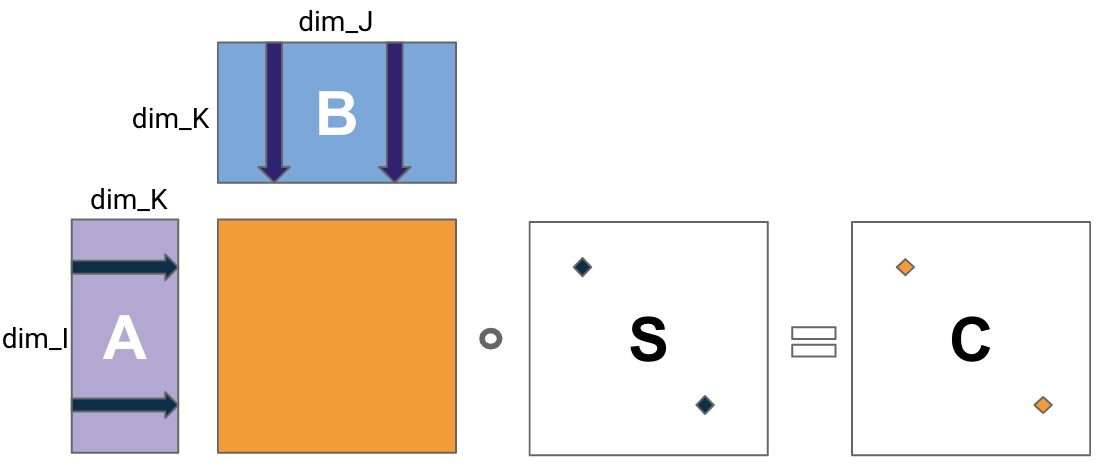
\includegraphics[width=0.9\linewidth]{fig/SDDMM-basic.png}
%     \caption{Visualization of an SDDMM operation. The arrows mark rows and columns of $A$ and $B$ which correspond to non-zero elements of the sampling matrix $S$.}
%     \label{fig:sddmm-basic}
% \vspace{-0.3cm}
% \end{figure}

% \hl{
% An efficient implementation of the algorithm would therefore skip regions in which the values of the sampling matrix $S$ are zero.
% %By identifying the non-zero elements of matrix $S$, we can compute only those rows and columns of A and B that correspond to those non-zero elements.
% By detecting the indices of these nonzero elements of $S$, programmers can use Gemmini's low-level programming interface to skip both the data movement and computation of the zero regions, while only invoking matrix multiplication at the non-zero regions. With Gemmini's low-level programming interface, programmers can load and operate on arbitrarily small pieces of data.
% By contrast, many higher-level programming interfaces expect large matrices as inputs, and are optimized for long-latency, high-throughput operations, which would not be suitable in such a sparse scenario.
% % Since Gemmini's smallest predication granularity is the spatial array dimension, an additional small bitmask can be applied to the computed results when they are moved back from the accelerator to the host processor.
% }

% \hl{
% We evaluate this approach using sparse sampling matrices from the Large Network Collection~\cite{snapnets} and Network Repository~\cite{networkrepo}. To explore a range of sampling density patterns, we evaluate two matrices with a low-density factor of less than 0.01\%, as well as a pair of sampling matrices with higher density factors of 2.5\% and 1.8\%. %Table~\ref{tab:sddmm_dataset} lists the sampling matrices dataset.
% The matrices are stored in Compressed Sparse Row (CSR) format~\cite{SpMV_CSR}.
% %Using the CSR row index pointer array, it is easy to identify which rows hold nonzero data. The exact nonzero data coordinate (i,j) can be determined by using the column indices array.
% For every non-zero element of $S$, we invoke Gemmini's fine-grained, low-level API to move the data and perform matrix multiplication.
% }

% \begin{table}[h!]
% \begin{center}
% \begin{tabular}{ p{2.1cm}||r |r|r|r  }
%  \hline
%  Dataset& Rows & Columns & \makecell{Non-zero\\Elements} & Density ($\%$)\\
%  \hline\hline
%  email-Eu-core & 1,005 & 1,005 & 25,571 &2.53\\
%  socfb-Amherst41 &2,235 & 2,235 & 90,954 & 1.82\\
%  scc\_rt\_lolgop & 9,742 & 9,742 & 9,020& 0.0095\\
%  scc\_rt\_gmanews&8,330&8,330&2,156&0.0031\\
%  \hline
% \end{tabular}
% \end{center}
% \caption{Dataset for sparse sampling matrix $S$.}
% \label{tab:sddmm_dataset}
% \end{table}

% Therefore, most rows and columns of A and B matrices would have to move in and compute, which end up only adding indirection overhead without effectively skipping anything.

% \hl{
% %The density and sparsity patterns of the sampling matrix S impact the optimal dimensions of the Gemmini spatial array.
% %We notice that the sparsity-pattern in the sampling matrices that were evaluated was such that a very fine-grained spatial array was required in order to identify zero-blocks at a DIM$\times$DIM granularity. Therefore, the kernel was evaluated with a Gemmini spatial array dimension of 4$\times$4.
% Figure~\mbox{\ref{fig:sddmm-perf}} shows performance comparisons of the SDDMM kernels with Gemmini's mid-level and low-level APIs across different datasets running on a Gemmini-generated accelerator with a 4$\times$4 spatial array. The results are normalized to the CPU performance running the same dataset.
% The mid-level API provides only an optimized dense matrix multiplication, while the low-level APIs give programmers the full control to skip unnecessary computation and data movement.
% Compared to the CPU baseline, we notice although the accelerator outperforms the CPU baseline for relatively dense datasets, CPU performs significantly better for the extremely sparse cases, especially compared to mid-level APIs.
% The reason for that is because of the non-trivial overhead of invoking accelerators and shuffling data in and out of accelerators.
% In addition, when the dataset is extremely sparse with less than $0.001\%$ density, CPU can operate directly at the scalar level for the dense region while our accelerator has to operate at the spatial-array granularity.
% }

% \hl{
% Comparing the mid- and low-level API performance, Figure~\mbox{\ref{fig:sddmm-perf}} shows that the low-level API outperforms the mid-level API by 306$\times$ for the extremely sparse matrices and 1.8$\times$ for the relatively dense ones. % (the high-level ONNX API was not evaluated since SDDMM is not an ONNX DNN operator.
% %The sampling matrices with the lowest-density factors exhibit a 306$\times$ performance improvement compared to the mid-level programming API, while sampling matrices with the higher density factors (density $>$ 1.5\%) only show 1.8$\times$ performance improvement.
% This is because the higher-density sampling matrices still have to absorb the overhead of the CSR data-structure traversal, but are not able to leverage the fine-granularity of the low-level API to skip zero regions due to the higher density.
% The results demonstrate that by using Gemmini's low-level programming interface, we are able to skip data movement and computation efficiently by using of fine-grained, small-granularity instructions which we could not have done efficiently if only high-level APIs were available.
% }
